% This version of CVPR template is provided by Ming-Ming Cheng.
% Please leave an issue if you found a bug:
% https://github.com/MCG-NKU/CVPR_Template.

%\documentclass[review]{cvpr}
\documentclass[final]{cvpr}

\usepackage{times}
\usepackage{epsfig}
\usepackage{graphicx}
\usepackage{amsmath}
\usepackage{amssymb}

% Include other packages here, before hyperref.

% If you comment hyperref and then uncomment it, you should delete
% egpaper.aux before re-running latex.  (Or just hit 'q' on the first latex
% run, let it finish, and you should be clear).
\usepackage[pagebackref=true,breaklinks=true,colorlinks,bookmarks=false]{hyperref}


\def\cvprPaperID{****} % *** Enter the CVPR Paper ID here
\def\confYear{CVPR 2021}
%\setcounter{page}{4321} % For final version only


\begin{document}

%%%%%%%%% TITLE
\title{Using Variable Length Google Search Volume Time-Series to Predict Natural
    Gas Prices with LSTMs}


\author{Quinn Murphey\\
University of Texas at San Antonio\\
1 UTSA Circle San Antonio, TX\\
{\tt\small quinn.murphey@my.utsa.edu}
% For a paper whose authors are all at the same institution,
% omit the following lines up until the closing ``}''.
% Additional authors and addresses can be added with ``\and'',
% just like the second author.
% To save space, use either the email address or home page, not both
\and
Adrian Ramos\\
University of Texas at San Antonio\\
1 UTSA Circle San Antonio, TX\\
{\tt\small adrian.ramos@my.utsa.edu}

\and
Gabriel Soliz\\
University of Texas at San Antonio\\
1 UTSA Circle San Antonio, TX\\
{\tt\small gabriel.soliz@my.utsa.edu}
}

\maketitle


%%%%%%%%% ABSTRACT
\begin{abstract}
    The ability to accurately project the price of commodities is one of the
    most useful applications of deep learning. It finds use from hedge funds
    seeking to maximize profit to public administrations modelling the outcomes
    of different policies. In the typical year, these algorithms are quite 
    successful, at least more so than their human counterparts. However, these
    models have almost always failed to predict drastic economic downturns such
    as the crash of oil in 2020 or the now expected crashes of Bitcoin.
    It’s critical to everyone that we can prepare for sudden events that can
    drastically alter the markets. Building off of the work of Tang et al.
    \cite{tang}, we use historical commodity prices along with Google
    search trends and news report sentimentatlity to hopefully achieve better
    commodity price predictions both in normal and abnormal times. In order
    to accomplish this task, we will use stacked LSTMs and BiLSTMs and perform a
    Bayesian search over the models hyperparameters. We will compare our results
    with those from similar papers.
\end{abstract}

%%%%%%%%% BODY TEXT
%~~~~~~~~~~~~~~~~~~~~~~~~~~~~~~~~~~~~~~~~~~~~~~~~~~~~~~~~~~~~~~~~~~~~~~~~~~~~~~~
\section{Introduction}

    The price fluctuation of good and stocks are often difficult to predict due
    to the numerous amounts of variables that play an important role of the
    price function. While there exists research that reflects on those expected
    variables \cite{romero}. Additionally, the research conducted which compares
    multiple results comprised from other researchers and their unique test
    leading to their results \cite{srivastava}.  The importance of being able to
    accurately predict the price of commodities is vital to creating plans to
    aid those in need. The more accurate our forecasting ability is, the better
    prepared we can hope to be in uncertain times. It would allow emergency
    services and first responders to allocate enough supplies in the event of
    unpredictable events that could cause server damage to our infrastructure.
    However, there has been minimal research on the price fluctuation of goods
    and stocks due to external events, such as war, pandemics, or environmental
    catastrophes. While reports have been brought up that show certain effects
    of specific tragedies, such as the COVID-19 pandemic report \cite{mead}. The
    rate that prices fluctuate of goods and stocks during times of crisis and
    compared to other times of crisis could potentially help uncover areas which
    are most impacted. Including opportunities for potential preventive measures
    to attempt to thwart a severe effect.

    The source code for our project can be found at 
    \url{https://www.github.org/Nragis/cs4263-project}.

%~~~~~~~~~~~~~~~~~~~~~~~~~~~~~~~~~~~~~~~~~~~~~~~~~~~~~~~~~~~~~~~~~~~~~~~~~~~~~~~
\section{Related Work}

    Our work builds off of a sequence of papers, all working on the NYMEX 
    natural gas prices dataset. 
    
    In their paper, Su et al., 2019 \cite{su} present the application of four 
    different machine learning algorithms including Gaussian process regression
    (GPR), gradient boosting machines (GBM), support vector machines (SVN) and 
    artificial neural networks (ANN) for the monthly prediction of natural
    gas spot prices.

    Building off of the work of Su et al., Ali, 2020 \cite{ali2020} and Ali et 
    al., 2021 \cite{ali2021} test out two more algorithms, LSBoost and a deep
    neural network (DNN) respectively. Both of these models, specifically the 
    DNN far outperformed the four models proposed by \cite{su}.

    Finally, Tang et al, 2019 \cite{tang} takes an alternative improvement on
    the work of \cite{su}. In their paper, they use a similar shallow ANN model,
    but they significantly improve the data used by using sentiment analyzed 
    yahoo finance articles and daily google search volume for "Natural Gas". 
    In a direct self-comparison, they found that the model given the google 
    search volume history far outperformed the model with only historical 
    prices data and the model that also had sentiment analyzed yahoo finance
    articles. Finally, Tang et al.'s work was on the four futures prices rather
    than the spot price.

%~~~~~~~~~~~~~~~~~~~~~~~~~~~~~~~~~~~~~~~~~~~~~~~~~~~~~~~~~~~~~~~~~~~~~~~~~~~~~~~
\section{Proposed Approach}

    In this paper, we combine the methods used in the papers above along with
    a few additions to produce a model that can accurately predict Natural Gas
    futures prices a day into the future. We will combine the data improvements
    of \cite{tang} and the model improvements of \cite{ali2021} to produce 
    results far outperforming either work. In addition, we will make 
    improvements on top of both papers in both categories.

    We will utilize variable time-length time series features to predict fixed
    time-length labels. Our features will span all the prior data that we have,
    rather than being restricted by a time-window. To help us predict futures
    prices, we will include historical natural gas futures and spot prices.
    Additionally, we will use google search volumes for terms we chose related
    to "Natural Gas" in order to demonstrate public interest in a topic over
    time.

    Finally, we will use LSTMs rather than simple feed forward perceptrons to
    perform a more powerful analysis on the time-series features. Following 
    these LSTMs, we will have a dense feed forward network to process the output
    of the LSTM layers.

%~~~~~~~~~~~~~~~~~~~~~~~~~~~~~~~~~~~~~~~~~~~~~~~~~~~~~~~~~~~~~~~~~~~~~~~~~~~~~~~
\section{Data}

\subsection{Labels}

    To be able to compare directly with Tang et al. \cite{tang}, we will use the
    same daily NYMEX natural gas futures prices from the US Energy Information
    Administration website (\url{https://www.eia.gov/}). These futures are for 1
    month, 2 month, 3 month, and 4 month time periods. In alignment with Tang,
    we will be using data from these four contracts from January 2013 to June
    2019. 1,638 records in total. Then, we will use simple linear interpolation 
    to fill in any days without an entry like weekends or holidays. We end up 
    with data from every day between January 2, 2013 to June 28, 2019, or 2,369 
    records total.

    \begin{figure}[h]
        \caption{Data descriptions of NYMEX futures prices from Jan 2, 2013 to
            June 28, 2019.} 
        \center
        \begin{tabular}{| c || c | c | c | c |}
            \hline 
            & Mean & Std Dev & Skew & Kurtosis\\ 
            \hline
            \hline
            Futures 1 & 3.172 & 0.718 & 0.637 &  0.202\\
            Futures 2 & 3.302 & 0.683 & 0.501 & -0.405\\
            Futures 3 & 3.232 & 0.660 & 0.461 & -0.540\\
            Futures 4 & 3.249 & 0.637 & 0.491 & -0.492\\
            \hline
        \end{tabular}
    \end{figure}

    Finally, we take the logarithm of every data point to eliminate the
    exponential nature of financial data and standardize each column seperately
    using following equations for each element
    \begin{equation}
        x' = \frac{(x-\mu)}{\sigma}
    \end{equation}
    where $\mu$ is the mean of the column and $\sigma$ is the standard 
    deviation.

    \begin{figure}[h]
        \caption{Data descriptions of regularized NYMEX futures prices from Jan 
            2, 2013 to June 28, 2019}
        \center
        \begin{tabular}{| c || c | c | c | c |}
            \hline 
            Regularized & Mean & Std Dev & Skew & Kurtosis\\ 
            \hline
            \hline
            Futures 1 & 0 & 1.0 & 0.033 & -0.087\\
            Futures 2 & 0 & 1.0 & 0.026 & -0.334\\
            Futures 3 & 0 & 1.0 & 0.040 & -0.475\\
            Futures 4 & 0 & 1.0 & 0.091 & -0.499\\
            \hline
        \end{tabular}
    \end{figure}

\subsection{Features}

\subsubsection{NYMEX}

    We will be using historical data from the same NYMEX dataset mentioned above
    including the natural gas spot prices we did not use for our labels. 
    However, we will nnow be using data ranging from January 5, 2004 to June 28,
    2019, filling empty days using the same interpolation methods. We end up 
    with 5,654 records of data, each with five points: one spot price and four 
    futures prices. See Figure \ref{fig:nymex_graph} for our graph of the NYMEX 
    dataset.

    We then regularize the data exactly as we did to our label data.
    
    \begin{figure*}[h]
        \caption{NYMEX Futures Prices from Jan 5, 2004 to June 28, 2019. \
            Labels in orange and features in both blue and orange.} 
        \center
        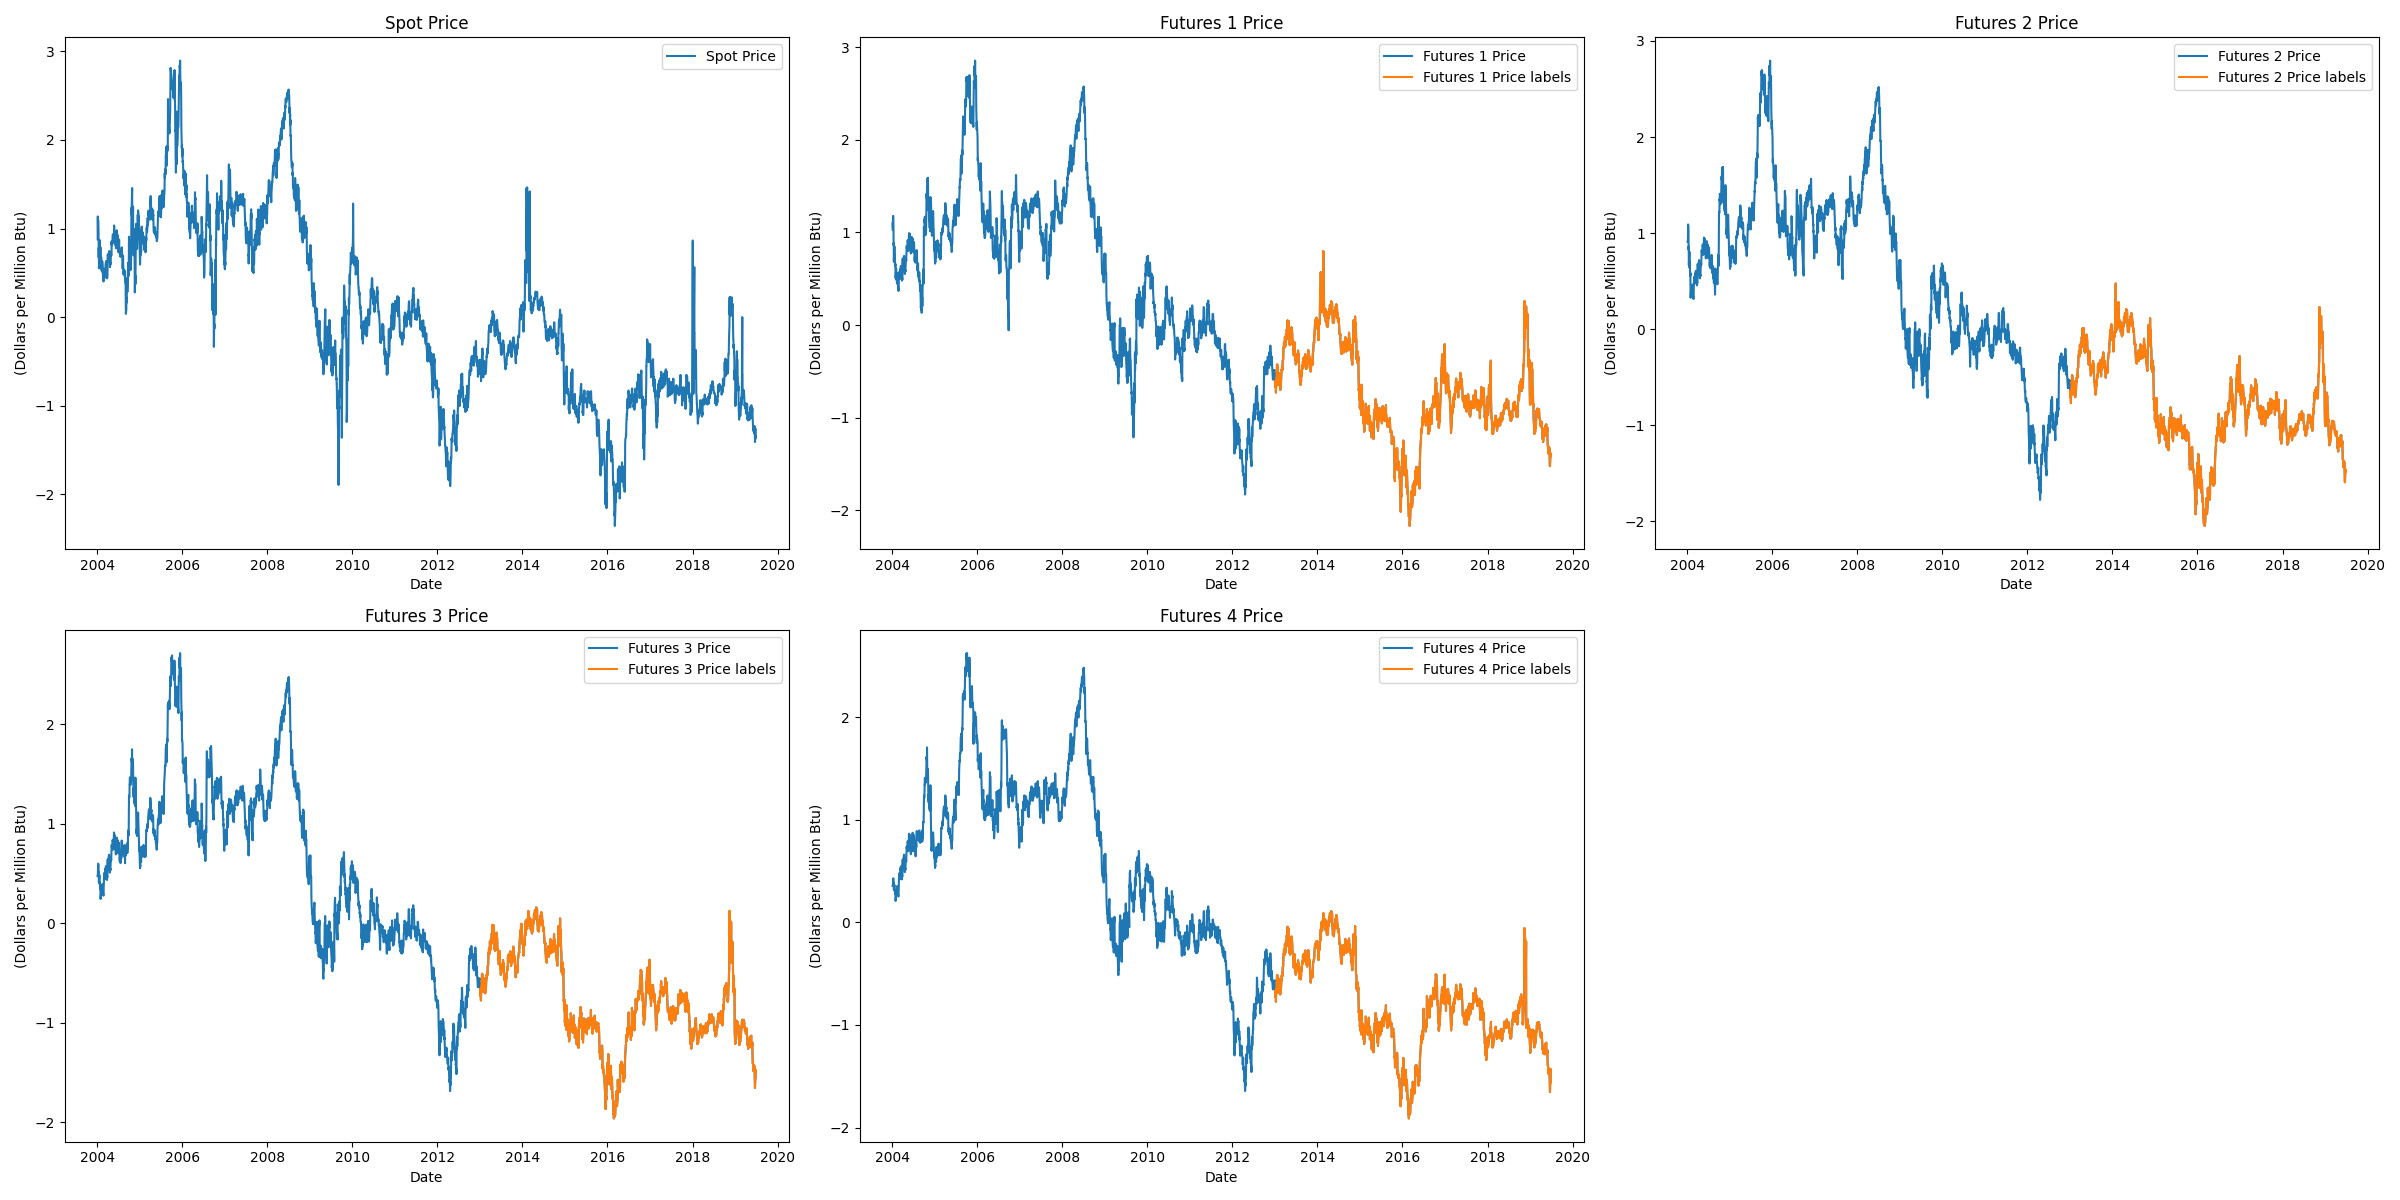
\includegraphics[width=1.0\textwidth]{images/nymex_data.png}
        \label{fig:nymex_graph}
    \end{figure*}
    
\subsubsection{Google Trends}

    We will be using Google Trends (\url{https://trends.google.com/}) as our
    source for Google search history data.  In this paper, we will be using the
    daily search volume data of 14 different terms, including "Natural Gas" from
    January 5, 2004 to June 28, 2019. We end up with the same number of 5,654
    records as we saw in our NYMEX features. However, for our google trends
    dataset, we have 14 columns, one for each search term. See Figure 
    \ref{fig:google_trends_desc} for data descriptive statistics and Figure 
    \ref{fig:google_trends_graph} for each series plotted (by the month). 
    
    Each column is not directly comparable with the other columns, and is only
    comparable with itself. For example, if "Natural Gas" has 23 for a day while
    "Recession" has a 73, this does not mean that "Recession" was searched more
    that day. This only means that "Recession" was searched more on this day
    than a day where "Recession" is less than 73.

    \begin{figure}[h]
        \caption{Data descriptions of daily Google search volume from Jan 5, 
            2004 to June 28, 2019.} 
        \center
        \begin{tabular}{| c || c | c | c | c |}
            \hline 
            & Mean & Std Dev & Skew & Kurtosis\\ 
            \hline
            \hline
            Natural Gas   & 51.95 & 10.62 &  0.181 &  0.758\\
            Oil           & 44.42 & 0.683 &  0.374 & -0.898\\
            Coal          & 24.19 & 0.660 &  0.368 &  0.276\\
            Nuclear Power & 5.662 & 4.064 &  7.544 &  135.1\\
            Wind Power    & 20.34 & 13.15 &  1.396 &  2.496\\
            Hydroelectric & 15.68 & 12.59 &  0.852 &  0.424\\
            Solar Power   & 35.28 & 12.69 &  0.676 &  0.697\\
            Gold          & 40.15 & 13.01 & -0.040 &  0.627\\
            Silver        & 47.10 & 10.54 & -0.224 &  0.176\\
            Platinum      & 43.51 & 8.671 &  0.325 &  1.355\\
            Copper        & 58.34 & 12.92 &  0.015 & -0.237\\
            Biofuel       & 12.82 & 12.15 &  1.762 &  4.112\\
            Recession     & 5.728 & 6.258 &  3.348 &  16.91\\
            CPI           & 20.55 & 11.41 &  1.031 &  1.893\\
            \hline
        \end{tabular}
        \label{fig:google_trends_desc}
    \end{figure}

    \begin{figure*}[h]
        \caption{Monthly Google search volume from Jan 5, 2004 to June 28, 2019}
        \center
        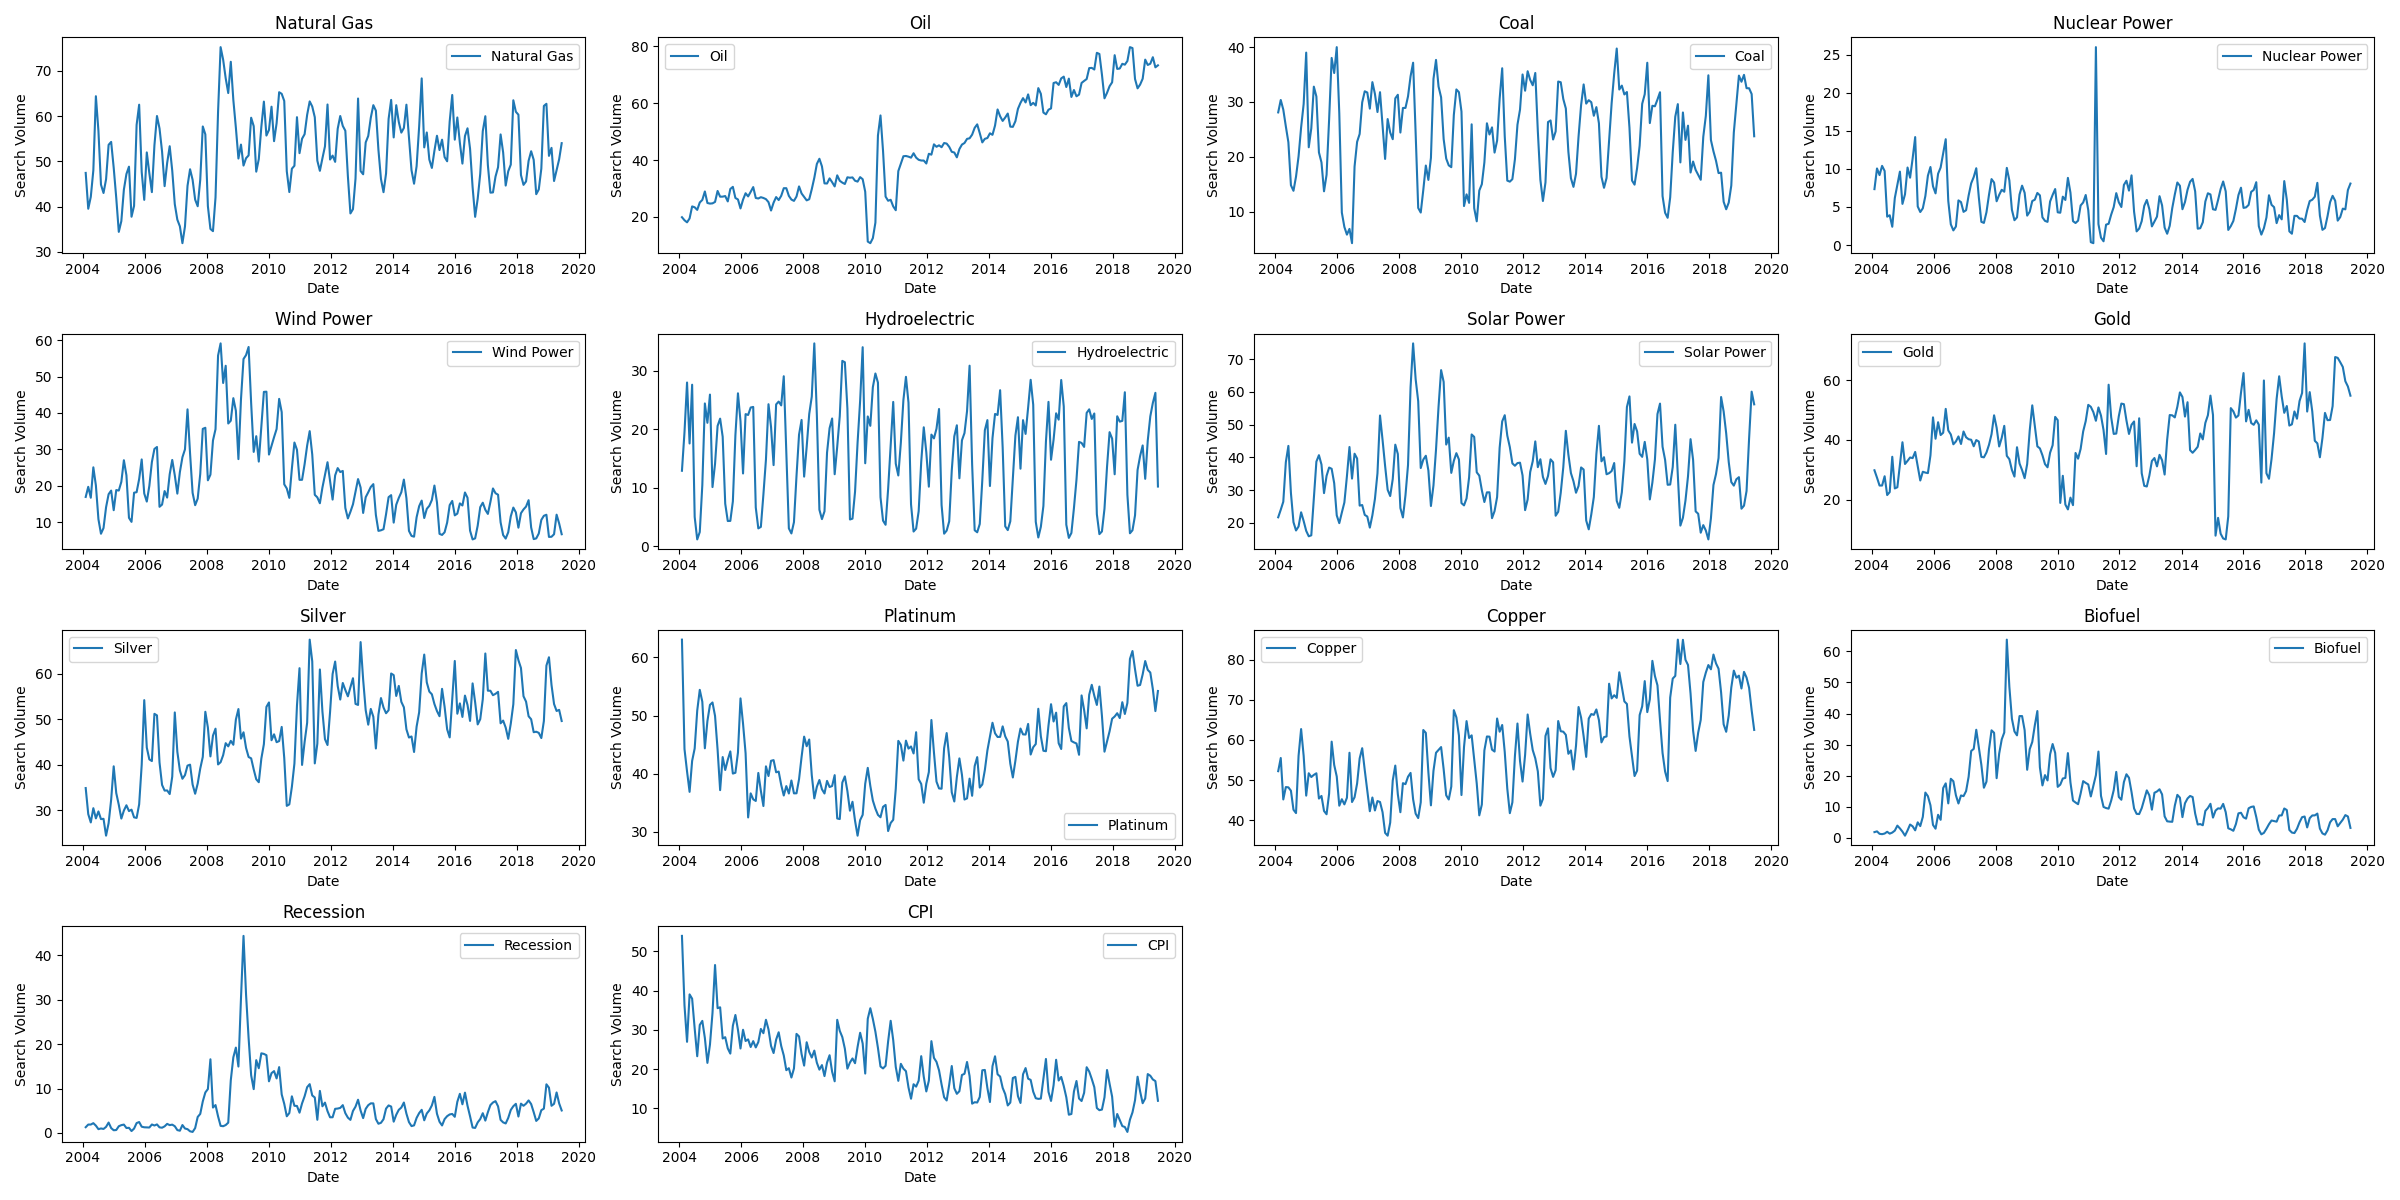
\includegraphics[width=1.0\textwidth]{images/google_trends_data_monthly.png}
        \label{fig:google_trends_graph}
    \end{figure*}

   
\subsection{Formatting Data}

    Instead of our features consisting of one or N days prior to the day we're 
    trying to predict (our label) using a time-series window. We will be using
    variable length time series features spanning from the beginning of our 
    dataset to the day immediately prior to our label. This allows us to have
    as much information as possible, given our datasets, for each prediction.

    The input to our model will look like $(Batch, Time, Features)$ where
    $Batch$ is fixed at 16, $Time$ is variable, and $Feature$ is fixed at 19 (5
    NYMEX and 14 Google).

    The output of our model will be fixed however, looking like $(Batch, 1, 
    Labels)$ where $Batch$ is 16, and $Labels$ is 4 (NYMEX Futures).

%~~~~~~~~~~~~~~~~~~~~~~~~~~~~~~~~~~~~~~~~~~~~~~~~~~~~~~~~~~~~~~~~~~~~~~~~~~~~~~~
\section{Metrics}

    In alignment with Tang, we will use mean absolute error (MAE) and root mean
    square error (RMSE) to compare results. Our goal is to minimize these
    values, indicating a more accurate regression.

    \begin{equation}
        MAE = \frac{1}{N}\sum_i^N|y_i - \hat{y_i}| \\
    \end{equation}

    \begin{equation}
        RMSE = \sqrt{\frac{1}{N}\sum_i^N(y_i - \hat{y_i})^2}
    \end{equation}

    Where $y_i$ and $\hat{y_i}$ are the real and predicted values respectively.

%~~~~~~~~~~~~~~~~~~~~~~~~~~~~~~~~~~~~~~~~~~~~~~~~~~~~~~~~~~~~~~~~~~~~~~~~~~~~~~~
\section{Results}

    We used Python3 for all of our code. We used Pytrends for scraping Google
    Trends data, and we use Pandas \cite{pandas} for our data formatting and
    preprocessing stages of our research. Finally, we used Keras \cite{keras},
    and Tensorflow \cite{tensorflow} for creating, training, and testing our
    models. Finally, we used Matplotlib \cite{matplotlib} to create all of our
    plots.

    We used a Tensorflow Dataset from generators rather than RaggedTensors to
    get variable time length tensors from our dataset and handle
    batching/shuffling. We also used 80\% of the data for training, 10\% for
    validation, and 10\% for testing in order to help prevent under/overfitting
    and select the best model.
    
    We experimented with both stacked LSTMs and stacked BiLSTMs followed by 
    several layers of densely connected perceptrons, and finally an output layer
    with a Mean-Squared-Error loss function. To find the best model for our
    data, we performed a Bayesian hyperparameter optimization using Keras Tuner
    \cite{kerastuner} over the hyperparameter dimensions listed in Figure
    \ref{fig:hyperparameters}). We ran this search for 50 trials, and let each
    model train for 50 epochs a piece.

    \begin{figure}[h]
        \caption{Hyperparameter distrbutions searched for our models}
        \center
        \begin{tabular}{| c || c | c | c | c |}
            \hline 
            Name & Type & Min & Max & Distribution(Step) \\ 
            \hline
            \hline
            LSTM Layers   & Int   & 1   & 5    & Uniform(1)\\
            LSTM Nodes    & Int   & 32  & 256  & Uniform(32) \\
            Dense Layers  & Int   & 1   & 3    & Uniform(1)\\
            Dense Nodes   & Int   & 256 & 2048 & Uniform(256)\\
            Dropout Rate  & Float & 0   & 0.999& Uniform\\
            Learning Rate & Float & 1e-6& 1e-1 & Log\\
            Beta\_1       & Float & 0.8 & 0.999& Linear\\
            \hline
        \end{tabular}
        \label{fig:hyperparameters}
    \end{figure}

    \begin{figure}[h]
        \caption{Best hyperparamers found by search and overall training loss}
        \center
        \begin{tabular}{| c || c | c |}
            \hline 
            Name & Stacked LSTM & Stacked BiLSTM\\ 
            \hline
            \hline
            LSTM Layers   & 1 & 1\\
            LSTM Nodes    & 256 & 32\\
            Dense Layers  & 1 & 1\\
            Dense Nodes   & 2048 & 2048\\
            Dropout Rate  & 0.0 & 0.0\\
            Learning Rate & 3e-5 & 1e-2\\
            Beta\_1       & 0.8 & 0.8\\
            \hline
            \hline
            Loss          & 0.004 & 0.004\\
            \hline
        \end{tabular}
        \label{fig:optimal_hyperparameters}
    \end{figure}

    The best hyperparameters we found are shown in Figure
    \ref{fig:optimal_hyperparameters}. Note the lack of layers. We will discuss 
    this in Section 8.

    After finding the optimal hyperparameters, we let the model train for a 
    total of 250 epochs, and saved the model with the lowest validation loss.
    See Figure \ref{fig:loss_over_epochs} to see the training and validation 
    loss over training epochs.

    \begin{figure*}[h]
        \caption{Stacked BiLSTM 1-day NYMEX futures prices predictions compared 
            with their true values}
        \center
        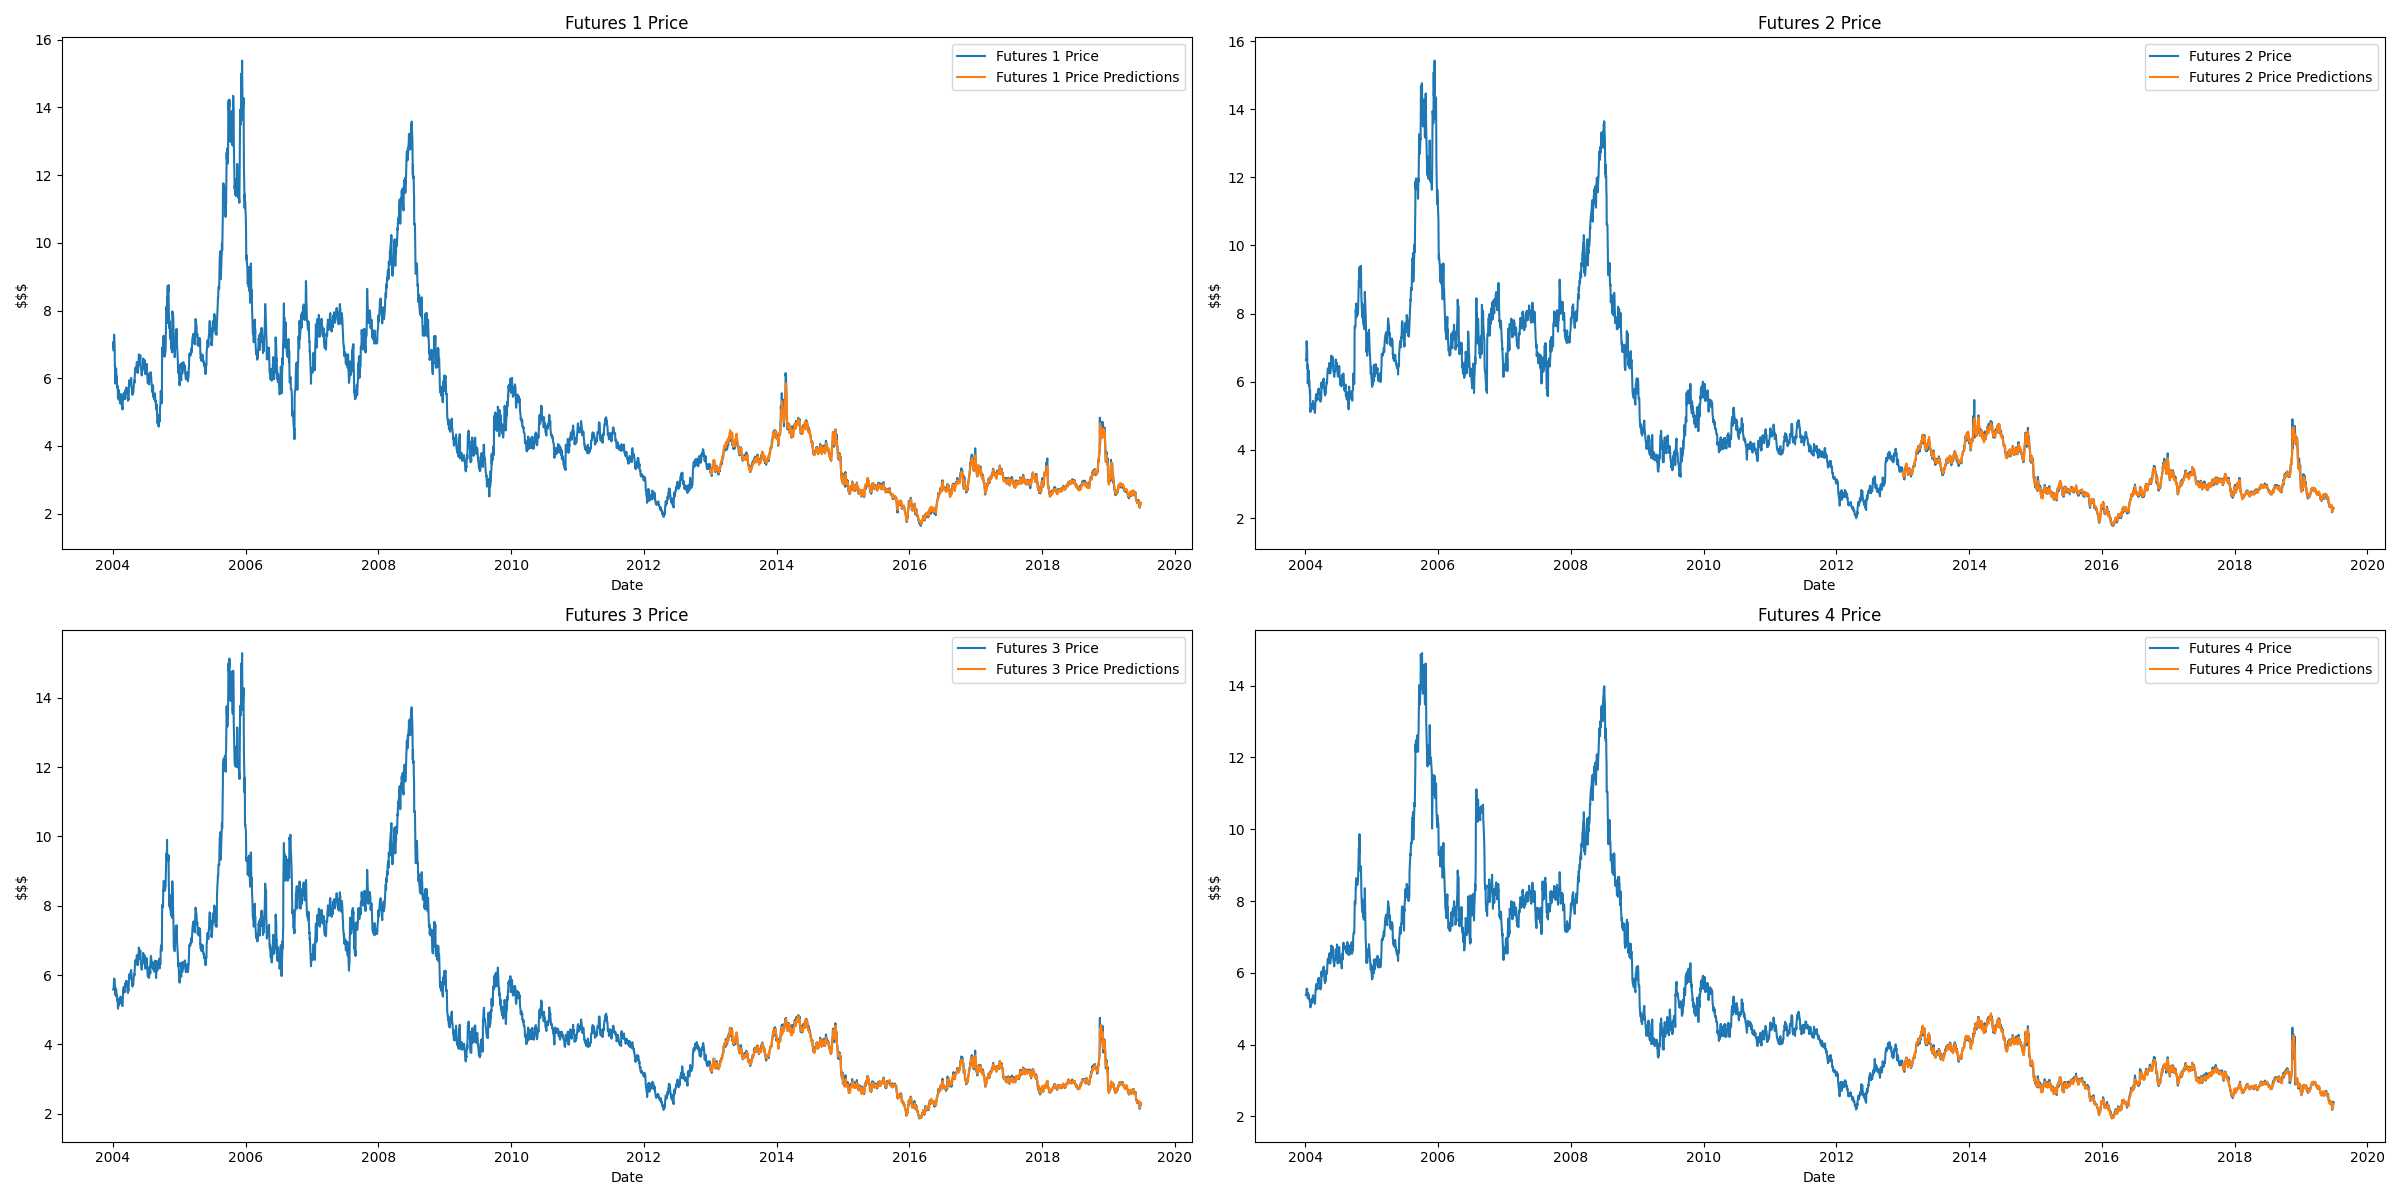
\includegraphics[width=1.0\textwidth]{images/stacked_bilstm_predictions.png}
        \label{fig:predictions_graph}
    \end{figure*}

    \begin{figure}[h]
        \caption{Training loss (blue) and validation loss (orange) over epochs
            trained of our Stacked BiLSTM model}
        \center
        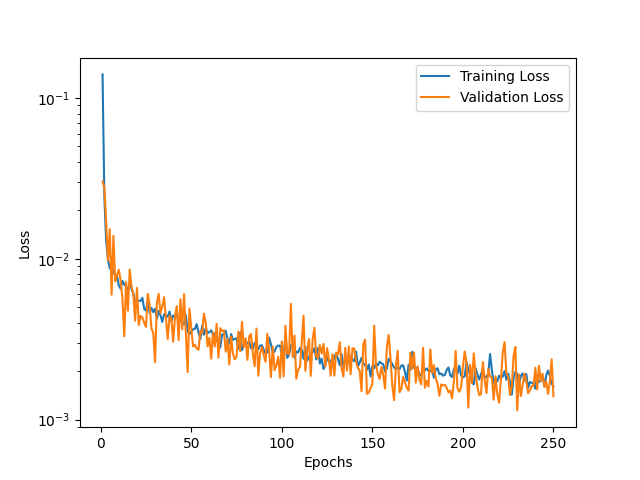
\includegraphics[scale=.51]{images/stacked_lstm_loss_over_epoch.png}
        \label{fig:loss_over_epochs}
    \end{figure}

    After training, we then tested these models on the test dataset we set aside
    previously, and evaluated the MAE and RMSE as shown above. The results are 
    in Figure \ref{fig:results}

    \begin{figure}[h]
        \caption{Comparison of Stacked LSTM to Stacked BiLSTM on predicting
            Natural Gas futures prices}
        \center
        \begin{tabular}{| c || c | c |}
            \hline
            Model & MAE & RMSE\\
            \hline
            \hline
            Stacked LSTM   & 0.0326 & 0.0435\\
            Stacked BiLSTM & 0.0261 & 0.0335\\
            \hline
        \end{tabular}
        \label{fig:results}
    \end{figure}
 
    Figure \ref{fig:predictions_graph} shows the predictions of our Stacked 
    BiLSTM model overlayed on top of the correct labels. As you can see, our 
    model is very close to exactly correct for most of the time-series. 
    Differing on average only 0.026 standard deviations from the correct value.

    
\section{Comparisons to Prior Work}

    We will be comparing our results with the results of the four other papers 
    mentioned in Section 2: Su et al. \cite{su}.  Ali et al., 2020
    \cite{ali2020}, Ali et al., 2021 \cite{ali2021}, and Tang et al.
    \cite{tang}.

    While, the first 4 all are predicting Natural Gas spot prices, Tang, like 
    us, is predicting Natural Gas futures prices. Thus, since Tang is 
    predicting 4 seperate data points, we must adjust their metrics accordingly:
    sum seperate MAEs for total MAE and square, sum, then root seperate RMSEs 
    for total RMSE.

    If we had more time, we would adapt out model to predict spot prices as well
    to directly compare to the first four papers better. However, since we do 
    not, we will multiply each MAE by four and each RMSE by two since they were
    metrics on a single length vector, while our metrics are on a length four
    vector. We do this to simulate the model having four identically good 
    outputs. This is not a perfect substitution by a long shot, but it allows
    us to compare our results more broadly.

    Finally, we take the best model from each paper for predicting one day 
    ahead. For this reason, we will only be comparing with our Stacked BiLSTM.

    The adjusted metrics from each paper next to our own can be found in Figure 
    \ref{fig:comparisons}.

    \begin{figure}[h]
        \caption{Comparison of Stacked LSTM to Stacked BiLSTM on predicting
            Natural Gas futures prices}
        \center
        \begin{tabular}{| p{2.5cm} | p{2cm} || c | c |}
            \hline
            Author & Model & MAE & RMSE\\
            \hline
            \hline
            Su et al. \cite{su}                 & ANN       & & 1.4494\\
            \hline
            Ali et al., 2020 \cite{ali2020}     & LSBoost   & & 1.1398\\
            \hline
            Ali et al., 2021 \cite{ali2021}     & DNN       & & 0.4880\\
            \hline
            Tang et al., 2021 \cite{tang}       & ANN       & 0.3663 & 0.2548\\
            \hline
            \hline
            This Study                      & BiLSTM & 0.0261 & 0.0355\\
            \hline
        \end{tabular}
        \label{fig:comparisons}
    \end{figure}

    As we can see above, our model performed much better than all the other 
    models. We performed over twice as good as even the prior best model.

    This improvement can likely be dually attributed to a stronger dataset,
    both from more google search terms, and from a variable time length feature,
    and to a stronger model, a stacked BiLSTM.

%~~~~~~~~~~~~~~~~~~~~~~~~~~~~~~~~~~~~~~~x~~~~~~~~~~~~~~~~~~~~~~~~~~~~~~~~~~~~~~~~
\section{Conclusion and Future Work}

    While our model performed quite well, we have already identified many ways
    in which it could be easily improved. 

    First, our computation power was limited, likely resulting in our optimal 
    lstm and dense depth being stunted below what they could be. We believe
    that with more computation time and power, a model with greater depth could
    outperform our model. This is supported by the fact that we didn't see even
    any overfitting in Figure \ref{fig:loss_over_epochs}.

    Second, the sentiment analysis used in Tang et al. could be used in 
    conjunction with google search volume to create an even more knowledgeable
    and hopefully superior model.

    Third, a search could be performed over all the top search trends to find 
    out which trends corrolate the strongest with the NYMEX prices. 
    Alternatively, one could perform a dimensionality reduction on a larger
    search volume dataset to feed directly into the model.

    Fourth, a seperate model could be created and trained for each of the labels
    (including spot price). This would allow the model to specialize more, and
    you could take the output of all 4 (or 5) of these models to get your 
    overall output.

    Finally, the ideas in this paper could be expanded to predict prices greater
    than one day in the future. Either, one could train a new model for each 
    time delta they would like to predict (1 day, 2 days, 3 days... ), or one
    could train a single model, and run a recursive calculation, concatentating
    the predictions for one day into the future onto the features, and feeding 
    that new time series into the model to predict two days into the future.

{\small
    \bibliographystyle{ieee_fullname}
    \bibliography{egbib}
}

\end{document}
